\chapter{Introduction to Neural Networks}\label{chp:1}
A \textbf{Neural Network} is a computational model inspired by the structure and functioning of the human brain. It consists of layers of interconnected nodes, called neurons, that process data in a manner similar to biological neurons. Neural networks are the foundation of \textbf{deep learning}, a subset of machine learning, and are used to recognize patterns, make predictions, and solve complex problems.

Key components of a neural network include:
\begin{itemize}
    \item \textbf{Input Layer}: Accepts the raw data for processing.
    \item \textbf{Hidden Layers}: Perform computations to extract patterns or features through weighted connections and activation functions.
    \item \textbf{Output Layer}: Produces the final result, e.g., classification or regression output.
\end{itemize}

Neural networks learn by adjusting the weights of connections between neurons using algorithms like \textbf{backpropagation}, minimizing the error between predicted and actual outputs. They are widely applied in tasks such as image recognition, natural language processing, and time-series forecasting.

\begin{figure}[h!]
    \centering
    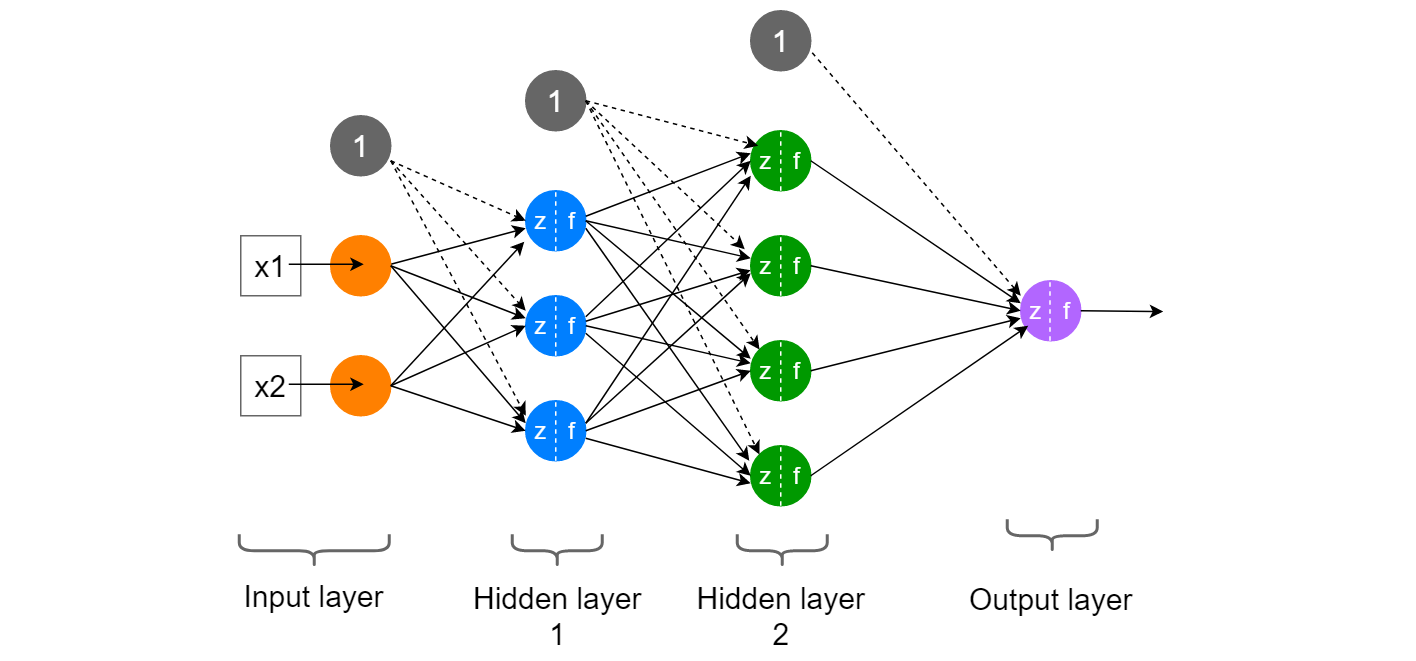
\includegraphics[width=\textwidth]{images/figure1.png}
    \caption{A typical Artificial Neural Network}
    \label{fig:1}
\end{figure}

\section{Background}
Artificial Neural Networks (ANNs) are computational models inspired by the structure and function of biological neural networks in the human brain. The idea of mimicking biological neurons dates back to the 1940s with the introduction of the \textbf{McCulloch-Pitts neuron model}, which laid the foundation for modern neural networks.\cite{mcculloch1943logical} Early research explored how networks of artificial neurons could compute logic functions and recognize patterns.\\

By the 1980s, the \textbf{backpropagation algorithm}, introduced by Rumelhart, Hinton, and Williams, marked a turning point by enabling efficient training of multi-layer networks.\cite{rumelhart1986learning} This innovation fueled interest in neural networks for tasks such as image recognition, speech processing, and robotics.\\

Despite their promise, neural networks struggled during the 1990s due to computational limitations and the dominance of simpler models like support vector machines (SVMs). However, the resurgence of interest in the 2010s, termed the \textbf{"deep learning revolution"}, was driven by three factors:
\begin{itemize}
    \item Availability of large datasets (e.g., ImageNet)
    \item Advancements in computational power (e.g., GPUs and TPUs).
    \item Development of new architectures and techniques, such as convolutional neural networks (CNNs) and recurrent neural networks (RNNs).\cite{lecun2015deep}\cite{krizhevsky2012imagenet}
\end{itemize}

\section{Applications of Neural Networks}
Neural networks are used across diverse domains, revolutionizing traditional methods with their ability to learn from data and generalize well. Prominent applications include:
\begin{itemize}
    \item \textbf{Image Recognition}: Tasks like facial recognition and object detection rely on CNNs to extract hierarchical features from images.\cite{lecun2015deep}
    \item \textbf{Natural Language Processing (NLP)}: Models like transformers power language models such as ChatGPT and BERT, enabling applications like sentiment analysis, translation, and summarization.\cite{vaswani2017attention}
    \item \textbf{Healthcare}: ANN-based solutions are applied for early diagnosis of diseases, drug discovery, and personalized treatment recommendations.\cite{esteva2017dermatologist}
    \item \textbf{Autonomous Systems}: Self-driving cars use neural networks to process sensor data for navigation and decision-making.\cite{bojarski2016end}
\end{itemize}

and many more...

\section{Importance of Neural Networks in Modern AI}
Neural networks form the backbone of modern AI, offering unparalleled flexibility and scalability for solving complex problems. Their key advantages include:
\begin{enumerate}
    \item \textbf{Automatic Feature Extraction}: Unlike traditional machine learning algorithms, ANNs can automatically learn hierarchical features from raw data.
    \item \textbf{Non-linearity}: Through activation functions, ANNs can model complex, non-linear relationships in data.
    \item \textbf{Scalability}: Modern architectures, such as deep neural networks, allow scaling to billions of parameters for solving real-world problems at scale.
\end{enumerate}

However, ANNs also have limitations, such as their need for large amounts of labeled data, computational intensity, and susceptibility to overfitting. Addressing these challenges remains a significant focus in the AI research community.\cite{goodfellow2016deep}

